\documentclass[12pt]{exam}
\usepackage[utf8]{inputenc}

\usepackage[margin=1in]{geometry}
\usepackage{amsmath,amssymb}
\usepackage{multicol}
\usepackage{mathrsfs}
\usepackage{graphicx}
\usepackage{multicol}
\usepackage[shortlabels]{enumitem}
\usepackage{scrextend}
\usepackage{xcolor}
\usepackage[normalem]{ulem}
\usepackage{optprog}
\usepackage{tikz}
\usepackage{calc}

\newcommand{\class}{SA405, Fall 2021}
\newcommand{\term}{}
\newcommand{\examnum}{Final Exam Practice}
\newcommand{\examdate}{}
\newcommand{\timelimit}{}

\pagestyle{head}
\firstpageheader{}{}{}
\runningheader{\class}{\examnum\ - Page \thepage\ of \numpages}{\examdate}
\runningheadrule

%% Answer box macros
%% \answerbox{alignment}{width}{height}
\newcommand{\answerbox}[3]{%
  \fbox{%
    \begin{minipage}[#1]{#2}
      \hfill\vspace{#3}
    \end{minipage}
  }
}

%% \answerboxfull{alignment}{height}
\newcommand{\answerboxfull}[2]{%
  \answerbox{#1}{6.38in}{#2}
}

%% \answerboxone{alignment}{height} -- for first-level bullet
\newcommand{\answerboxone}[2]{%
  \answerbox{#1}{6.0in}{#2}
}

%% special boxes
\newcommand{\wordbox}{\answerbox{c}{1.2in}{.7cm}}
\newcommand{\catbox}{\answerbox{c}{.5in}{.7cm}}
\newcommand{\letterbox}{\answerbox{c}{.7cm}{.7cm}}

\printanswers
%\noprintanswers

\begin{document}

\noindent
\begin{tabular*}{\textwidth}{l @{\extracolsep{\fill}} r @{\extracolsep{6pt}} r}
\textbf{\class} &&\textbf{\examnum}\\
\textbf{\term} &&\textbf{\examdate}\\

%\emph{Midshipmen are persons of integrity.}& \textbf{Name:} & \makebox[2.2in]{\hrulefill}\\\\
%\textbf{Time Limit: \timelimit} &  & \makebox[2in]{\hrulefill}
\end{tabular*}


\noindent
\rule[2ex]{\textwidth}{2pt}

%This exam contains \numpages\ pages (including this cover page) and \numquestions\ questions.\\
%Total of points is \numpoints.
\noindent Final exam guidance:
\begin{itemize}
%\item You may pull the pages apart and then staple them together at the end.  I prefer not to see your name when I am grading, so only write your name on the first page (unless submitting pages unstapled).
%
%\item No books, notes, or any other outside help % or calculators
%% that do symbolic manipulation (such as TI-89 or TI-92)
% allowed. %{\bf One} 8.5 by 11 inch formula/note sheet is allowed.
%
%%\item You may use your calculator on this test.
%
%\item Show work clearly and neatly.
%
%\item Define all notation used.
%%\item If you need more space than is provided, use the back of the previous page.
%
%\item Please read each question carefully.
%If you are not sure what a question is
%asking, ask for clarification.
%
%\item If you start over on a problem, please CLEARLY indicate what your final
%  answer is, along with its accompanying work.

\item  The SA405 final exam is on Tues 14 Dec at 755 on the first deck of Chauvenet Hall.  (Check mids for the exact classroom that your section is in.)
\item  You may bring in a single, two-sided, 8.5'' x 11'' sheet of notes that has been handwritten by you (no scanning or printing involved) to use during the exam.
\item  There will be no Python on the final exam.  All other material is fair game.
\item  \textbf{The practice problems on this document do NOT represent an exhaustive list of topics that may appear on the final exam.}
\item  To prepare for the final exam, you should study all tests, quizzes, homework problems,  and notes.  I would recommend reworking any problems that you aren't comfortable with after reviewing the notes for those topics.
\item Good luck!
\end{itemize}

%\bigskip
%\begin{center}
%Grade Table (for teacher use only)\\
%\addpoints
%\gradetable[v][questions]
%\end{center}

\noindent
\rule[2ex]{\textwidth}{2pt}

%\newpage %%%%%%%
\begin{questions}



\question Consider the following:
%\[
%z = \max  8 x_1 + 9 x_2 + 6 x_3 + 4 x_4
%\]
%s.t.
%\begin{equation}
%  \label{ip}
%  \notag
%  \begin{array}{rrrrll}
%  5 x_1 & + 7 x_2 & + 4 x_3 & + 3 x_4 & \leq & 67 \\
%  x_1, & x_2,  & x_3 & x_4 & \geq 0, ~ & x_1,x_2,x_3,x_4 \text{ are integer.}
%\end{array}
%\end{equation}%Note that $x_1,x_2,x_3,x_4 \in \mathbb{Z}$ means that $x_1,$  $x_2,$ $x_3$, and $x_4$ are integer variables.
CDR Could B. Wright is attempting to solve a \emph{maximizing} integer program using branch-and-bound.  All four variables, $x_1,$  $x_2,$ $x_3$, and $x_4$, are required to be nonnegative integers.
\vspace{0.2 cm}

\begin{parts}

  \part He begins by solving the problem as an LP-relaxation.  His solver returns the solution shown in the box labeled P1 below.

\begin{figure}[h]
  \centering
  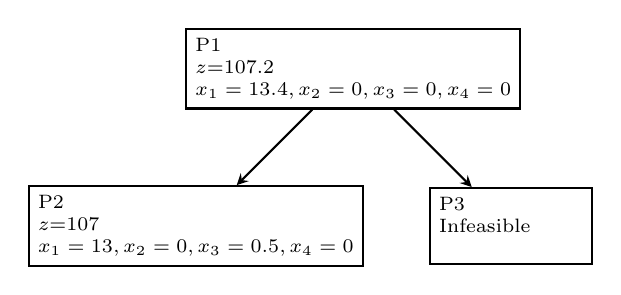
\begin{tikzpicture}
    [font=\scriptsize,
    node/.style={shape=rectangle,draw=black,minimum width=0.5cm,thick},
    arc/.style={->,>=stealth,thick},
    edge/.style={thick}]

   \node (P1) [node] at (0,0) {{\parbox{\widthof{$x_1=13.4, x_2=0, x_3 =0, x_4=0$}}{
    P1 \\
    $z$=107.2 \\
    $x_1 = 13.4, x_2=0, x_3=0, x_4=0$}}};

   \node (P2) [node] at (-2,-2) {{\parbox{\widthof{$x_1=13, x_2=0, x_3 =0.5, x_4=0$}}{
    P2 \\
    $z$=107 \\
    $x_1=13, x_2=0, x_3 =0.5, x_4 =0$}}};

   \node (P3) [node] at (2,-2) {{\parbox{\widthof{x=8.1667, y=2}}{
    P3 \\
    Infeasible  \\
    $ $}}};


    \draw [arc] (P1) -- (P2) node[pos=0.5,left] {}; %$x_1 \leq 13$} };
    \draw [arc] (P1) -- (P3) node[pos=0.5,right] {}; %$x_1 \geq 14$}};

  \end{tikzpicture}

\end{figure}
At the initialization phase (based on P1 only), what are the upper and lower bounds on the optimal integer solution, which we will denote $z^*$?
\begin{solution}
$-\infty < z^* \leq 107 = \lfloor 107.2 \rfloor$.  (The lower bound comes from an incumbent solution, and there is no incumbent solution yet.)
\end{solution}

\part He then chooses a variable to branch on and adds the appropriate inequalities to the model (you may assume he does this correctly).  Label both of the arcs from P1 with the branching variable and inequality that led to the solutions shown in the boxes labeled P2 and P3.

  \begin{solution}
  $x_1 \leq 13$, $x_1 \geq 14$
  \end{solution}

\part CDR Could B. Wright initially claims that he can stop using branch-and-bound at this point because he has found an integer objective value with subproblem P2.  Explain why this is not the case.

\begin{solution}
He should not terminate branch and bound at this point because he hasn't found a feasible integer SOLUTION ($x_3$ is not an integer), and P2 is still an active node that needs to be explored.
\end{solution}


\part CDR Could B. Wright takes your advice and continues using branch-and-bound and arrives at the tree shown below.  Label both of the arcs from P2 with the branching variable and inequality that led to the solutions shown in the boxes labeled P4 and P5.

\begin{figure}[h]
  \centering
  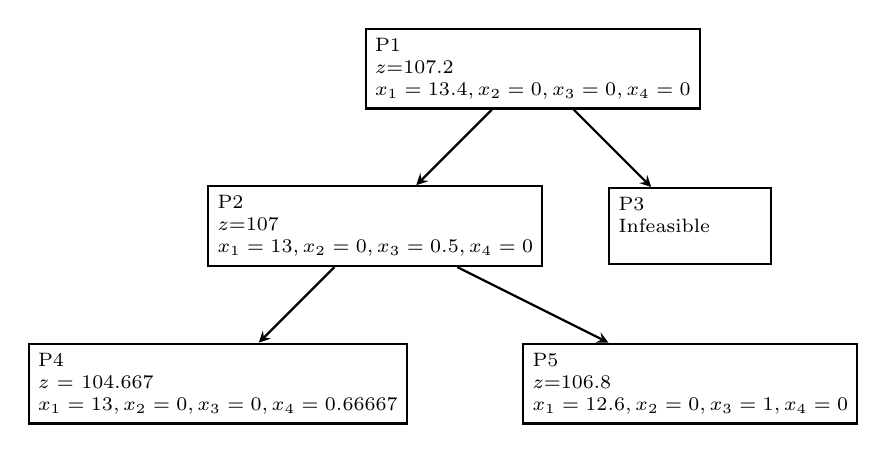
\begin{tikzpicture}
    [font=\scriptsize,
    node/.style={shape=rectangle,draw=black,minimum width=0.5cm,thick},
    arc/.style={->,>=stealth,thick},
    edge/.style={thick}]

   \node (P1) [node] at (0,0) {{\parbox{\widthof{$x_1=13.4, x_2=0, x_3 =0, x_4=0$}}{
    P1 \\
    $z$=107.2 \\
    $x_1 = 13.4, x_2=0, x_3=0, x_4=0$}}};

   \node (P2) [node] at (-2,-2) {{\parbox{\widthof{$x_1=13, x_2=0, x_3 =0.5, x_4=0$}}{
    P2 \\
    $z$=107 \\
    $x_1=13, x_2=0, x_3 =0.5, x_4 =0$}}};

   \node (P3) [node] at (2,-2) {{\parbox{\widthof{x=8.1667, y=2}}{
    P3 \\
    Infeasible  \\
    $ $}}};

   \node (P4) [node] at (-4,-4) {{\parbox{\widthof{$x_1=13, x_2=0, x_3 = 0, x_4 =0.66667$}}{
    P4 \\
    $z$ = 104.667  \\
    $x_1=13, x_2=0, x_3 = 0, x_4 =0.66667$}}};

   \node (P5) [node] at (2,-4) {{\parbox{\widthof{$x_1=12.6, x_2=0, x_3 = 1, x_4 =0$}}{
    P5 \\
    $z$=106.8 \\
   $x_1=12.6, x_2=0, x_3 = 1, x_4 =0$}}};


    \draw [arc] (P1) -- (P2) node[pos=0.5,left] { };
    \draw [arc] (P1) -- (P3) node[pos=0.5,right] { };
    \draw [arc] (P2) -- (P4) node[pos=0.5,left] {}; %{\begin{solution}$x_3 \leq 0$} };
    \draw [arc] (P2) -- (P5) node[pos=0.5,right] {}; %{\begin{solution}$x_3 \geq 1$} };

  \end{tikzpicture}
\end{figure}
\begin{solution}
$x_3 \leq 0$, $x_3 \geq 1$
\end{solution}
\part  What are the incumbent solution, global lower, and global upper bounds at this point in branch and bound?
\begin{solution}
There is no incumbent solution yet, so the current global lower bound is still $-\infty$.  The global upper bound is 106, which is the largest upper bound among the active subproblems (P4 and P5).
\end{solution}
\part If CDR Could B. Wright wants to use a Best-First Search approach, which subproblem should he choose to branch on next?  Briefly explain your answer for full credit.
\begin{solution}
He should branch on P5 because $106.8 > 104.667$.  Best-First Search means we branch on the subproblem with the largest objective value when we have a maximization objective function.
\end{solution}

\part CDR Could B. Wright continues using branch-and-bound and arrives at the tree shown below.

\begin{figure}[h]
  \centering
  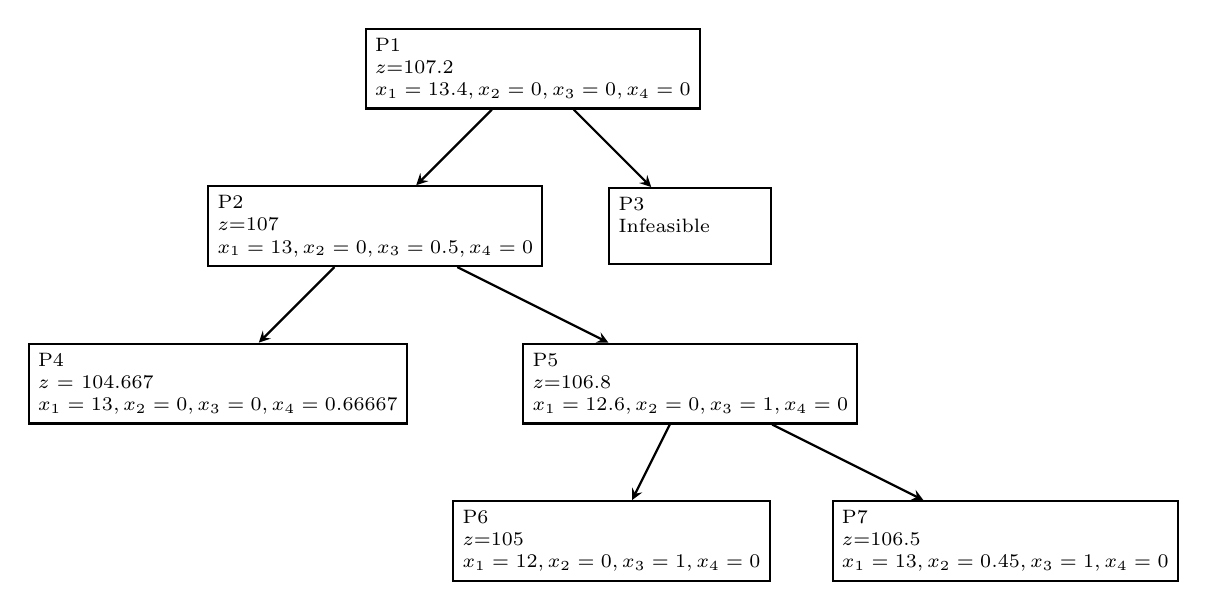
\begin{tikzpicture}
    [font=\scriptsize,
    node/.style={shape=rectangle,draw=black,minimum width=0.5cm,thick},
    arc/.style={->,>=stealth,thick},
    edge/.style={thick}]

  \node (P1) [node] at (0,0) {{\parbox{\widthof{$x_1=13.4, x_2=0, x_3 =0, x_4=0$}}{
    P1 \\
    $z$=107.2 \\
    $x_1 = 13.4, x_2=0, x_3=0, x_4=0$}}};

   \node (P2) [node] at (-2,-2) {{\parbox{\widthof{$x_1=13, x_2=0, x_3 =0.5, x_4=0$}}{
    P2 \\
    $z$=107 \\
    $x_1=13, x_2=0, x_3 =0.5, x_4 =0$}}};

   \node (P3) [node] at (2,-2) {{\parbox{\widthof{x=8.1667, y=2}}{
    P3 \\
    Infeasible  \\
    $ $}}};

{\node (P4) [node] at (-4,-4) {{\parbox{\widthof{$x_1=13, x_2=0, x_3 = 0, x_4 =0.66667$}}{
    P4 \\
    $z$ = 104.667  \\
    $x_1=13, x_2=0, x_3 = 0, x_4 =0.66667$}}};}

   \node (P5) [node] at (2,-4) {{\parbox{\widthof{$x_1=12.6, x_2=0, x_3 = 1, x_4 =0$}}{
    P5 \\
    $z$=106.8 \\
   $x_1=12.6, x_2=0, x_3 = 1, x_4 =0$}}};

   {\node (P6) [node] at (1,-6) {{\parbox{\widthof{$x_1=12, x_2=0, x_3 =1, x_4=0$}}{
    P6 \\
    $z$=105 \\
   $x_1=12, x_2=0, x_3 =1, x_4=0$}}};}

   \node (P7) [node] at (6,-6)  {{\parbox{\widthof{$x_1=12, x_2=0, x_3 =1.75, x_4=0$}}{
    P7 \\
    $z$=106.5  \\
    $x_1=13, x_2=0.45, x_3 = 1, x_4=0$}}};

    \draw [arc] (P1) -- (P2) node[pos=0.5,left] { };
    \draw [arc] (P1) -- (P3) node[pos=0.5,right] { };
    \draw [arc] (P2) -- (P4) node[pos=0.5,left] { };
    \draw [arc] (P2) -- (P5) node[pos=0.5,right] { };
    \draw [arc] (P5) -- (P6) node[pos=0.5,left] { };
    \draw [arc] (P5) -- (P7) node[pos=0.5,right] { };

  \end{tikzpicture}
\end{figure}
What are the incumbent solution, global lower bound, global upper bound, and MIP gap at this point in branch and bound?
\begin{solution}
Incumbent solution:  $(12,0,1,0)$.  $105 \leq z^* \leq 106$.  MIP gap $= \frac{|106-105|}{|105|} = 0.009$.
\end{solution}
\part  Label the status of each node as  active, branched, fathomed, or incumbent.
\begin{solution}
P1:  branched, P2: branched, P3: fathomed, P4: fathomed, P5: branched, P6: incumbent, P7: active
\end{solution}
\part  What should happen next in the algorithm?  If the algorithm should terminate, what is the optimal solution?  If the algorithm should continue, explain how the next subproblems are produced.
\begin{solution}
The algorithm should continue because there is still an active node: P7.  Branch at P7 on $x_2$.  Add the constraint $x_2 \leq 0$ to form P8, and add constraint $x_2 \geq 1$ to form P9.
\end{solution}

\end{parts}


\question  Draw two 2-dimensional shapes with straight edges, one convex and one nonconvex.  Explain your examples.
\begin{solution}
\end{solution}
\newpage
\question Consider the following integer linear program:
\[
\max  3 x_1 + 14 x_2 + 18 x_3
\]
s.t.
\begin{equation}
  \label{lp}
  \tag{$P$}
  \begin{array}{rrrcr}
  3 x_1 & + 5 x_2 & + 6 x_3 & \leq & 10 \\
  x_1, & x_2, & x_3 & \in & \{0,1\}
\end{array}
\end{equation}
whose linear programming relaxation optimal solution is $x_1 = 0$, $x_2 = \frac{4}{5}$, and $x_3 = 1$.

\vspace{0.2 cm}
\noindent Recall the following definitions:
\begin{itemize}
\item A linear inequality is a \textbf{valid inequality} for a given discrete optimization model if it holds for all (integer) feasible solutions to the model.
\item To \textbf{strengthen} a relaxation, a valid inequality must cut off (render infeasible) some feasible solutions to the current linear programming relaxation that are not feasible in the full integer linear programming model.
\end{itemize}

\bigskip
\begin{parts}

\part The inequality $x_1 + x_2 + x_3 \leq 1$ is (circle one):
 {\bf valid} or {\bf not valid}
\newline for this model.  Briefly explain your answer for full credit.
\begin{solution}
The inequality is {\bf not valid}.  For example, the inequality does not hold for the feasible solution
$(1,1,0)$ of the IP.
\end{solution}

\part  Explain why the inequality $x_2 + x_3 \leq 1$ is valid for this model.
\begin{solution}
The inequality is valid because it holds for all feasible solutions of the IP. There are  six feasible solutions of the IP, $(0,0,0); (0,0,1); (0,1,0); (1,0,0); \\ (1,0,1); (1,1,0)$ (the triplets $(0,1,1); (1,1,1)$ are not feasible) and it is easy to check that they all satisfy the inequality $x_2 + x_3 \leq 1$.
\end{solution}

\part Adding the constraint $x_2 + x_3 \leq 1$  would (circle one):  {\bf strengthen} or {\bf not improve}
\newline the linear programming relaxation.  Briefly explain your answer for full credit.
\begin{solution}
Adding the constraint $x_2 + x_3 \leq 1$  would {\bf strengthen} the original LP relaxation. The optimal solution of the original LP relaxation, $x_1 = 0$, $x_2 = \frac{4}{5}$, and $x_3 = 1$,  does not satisfy  the constraint $x_2 + x_3 \leq 1$, hence,  part of the feasible region of the original LP relaxation  is ''cut off'' and the new LP relaxation  is ''tighter''.
\end{solution}

\end{parts}
\newpage


\question Consider the following graph. The numbers above the arcs are costs.

%This latex requires the tikz package
\begin{center}
  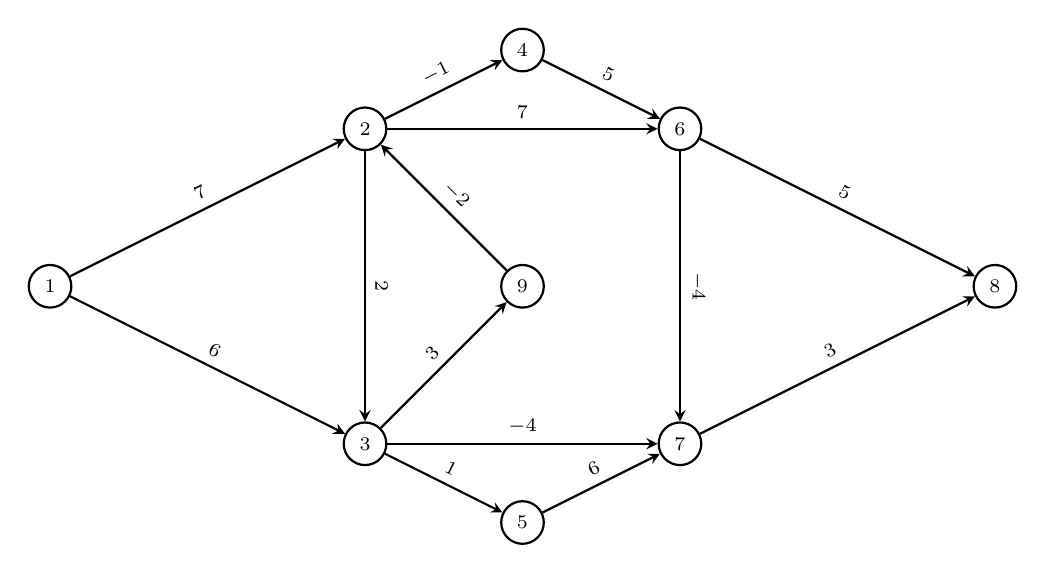
\begin{tikzpicture}
    [font=\scriptsize,
    node/.style={shape=circle,draw=black,minimum width=0.5cm,thick},
    arc/.style={->,>=stealth,thick},
    arclabel/.style={midway,sloped,above},
    edge/.style={thick}]

    \node (1) [node] at (-8,1) {1};
    \node (2) [node] at (-4,3) {2};
    \node (3) [node] at (-4,-1) {3};
    \node (4) [node] at (-2,4) {4};
    \node (5) [node] at (-2,-2) {5};
    \node (6) [node] at (0,3) {6};
    \node (7) [node] at (0,-1) {7};
    \node (8) [node] at (4,1) {8};
    \node (9) [node] at (-2,1) {9};

%    \node (11) [node,shape=rectangle,dashed] at (-8.7,1) {0};
%    \node (21) [node,shape=rectangle,dashed] at (-4,3.6) {M};
%    \node (31) [node,shape=rectangle,dashed] at (-4,-1.6) {M};
%    \node (41) [node,shape=rectangle,dashed] at (-2,4.6) {M};
%    \node (51) [node,shape=rectangle,dashed] at (-2,-2.6) {M};
%    \node (61) [node,shape=rectangle,dashed] at (0,3.6) {M};
%    \node (71) [node,shape=rectangle,dashed] at (0,-1.6) {M};
%    \node (81) [node,shape=rectangle,dashed] at (4.7,1) {M};
%    \node (91) [node,shape=rectangle,dashed] at (-1.3,1) {M};

    \draw [arc] (1) -- (2) node [arclabel] {$7$};
    \draw [arc] (1) -- (3) node [arclabel] {$6$};
    \draw [arc] (2) -- (3) node [arclabel] {$2$};
    \draw [arc] (2) -- (4) node [arclabel] {$-1$};
    \draw [arc] (3) -- (5) node [arclabel] {$1$};
    \draw [arc] (4) -- (6) node [arclabel] {$5$};
    \draw [arc] (3) -- (7) node [arclabel] {$-4$};
    \draw [arc] (2) -- (6) node [arclabel] {$7$};
    \draw [arc] (9) -- (2) node [arclabel] {$-2$};
    \draw [arc] (5) -- (7) node [arclabel] {$6$};
    \draw [arc] (6) -- (7) node [arclabel] {$-4$};
    \draw [arc] (6) -- (8) node [arclabel] {$5$};
    \draw [arc] (7) -- (8) node [arclabel] {$3$};
    \draw [arc] (3) -- (9) node [arclabel] {$3$};
  \end{tikzpicture}
\end{center}

\begin{parts}
\part  Formulate a concrete integer program whose solution provides the shortest paths from node 1 to each of the following nodes: 6, 8, and 9.
\begin{solution}

\begin{tabbing}
\noindent{\bf Decision Variables}\\[0.2cm]
$x_{i,j}$ number of times arc $(i,j)$  was used on shortest paths, \\
\hspace*{.7cm} for all $i,j \in \{1, \ldots, 9\}$ set of nodes  \\[0.2cm]
\end{tabbing}

\noindent{\bf Formulation}
\begin{alignat*}{3}
\min \quad & 7~x_{1,2} + 6~x_{1,3}+ \ldots + (-2)~x_{9,2}\\
\mbox{s.t.~~} & x_{1,2} + x_{1,3} = 3 &\qquad& \mbox{node 1, starting node} && \\
& x_{1,2} +x_{9,2}= x_{2,3}+x_{2,4} + x_{2,6} &\qquad& \mbox{ node 2, transitional node} && \\
& x_{1,3}+x_{2,3} = x_{3,5}+ x_{3,7}+ x_{3,9}  &\qquad& \mbox{ node 3, transitional node} && \\
& x_{2,4} = x_{4,6}  &\qquad& \mbox{ node 4, transitional node} && \\
& x_{3,5} = x_{5,7} &\qquad& \mbox{ node 5, transitional node} && \\
& x_{2,6}+x_{4,6}- x_{6,7}-x_{6,8} =1 &\qquad& \mbox{ node 6, destination node} && \\
& x_{3,7}+x_{5,7} + x_{6,7}  = x_{7,8}  &\qquad& \mbox{ node 7, transitional node} && \\
& x_{6,8}+x_{7,8} =1 &\qquad& \mbox{ node 8, destination node} && \\
& x_{3,9}-x_{9,2} =1 &\qquad& \mbox{ node 9, destination node} && \\
 & x_{i,j} \geq 0 &&  \\
\end{alignat*}


\end{solution}
\part  Convert your concrete model to abstract form.  Define all notation used.  Describe the purpose of the objective function and each constraint.
\begin{solution}

\begin{tabbing}
\noindent{\bf Sets}\\[0.2cm]
\hspace*{.5cm} \= $N$ \hspace{2cm} \= set of nodes\\
\> Node $1$ \>  starting node for any shortest path \\
\> $D\subseteq N-\left\{1\right\}$ \> destination nodes\\
\> $A$ \> set of arcs $(i,j)$ for $i,j \in N$  \\[0.2cm]
\noindent{\bf Parameters}\\[0.2cm]
\> $c_{i,j}$ \> the cost on the arc $(i,j) \in A$ \\[0.2cm]

\noindent{\bf Decision Variables}\\[0.2cm]
\> $x_{i,j}$ \> number of times arc $(i,j)\in A$  was used on shortest paths\\[0.2cm]
\end{tabbing}

\noindent{\bf Formulation}

\begin{alignat}{3}
\min \quad &  \sum_{(i,j )\in A} c_{i,j} x_{i,j} \\
\mbox{s.t.} \quad & \sum_{j \in N:(1,j )\in A} x_{1,j} - \sum_{i \in N:(i,1 )\in A} x_{i,1}=
\left|D\right| &\qquad&  \left|D\right| \mbox{ cardinality of set} D\\
\quad & \sum_{j \in N:(n,j )\in A} x_{n,j} - \sum_{i \in N:(i,n )\in A} x_{i,n}= 1 &\qquad&  \forall n \in D \\
\quad & \sum_{j \in N:(n,j )\in A} x_{n,j} - \sum_{i \in N:(i,n )\in A} x_{i,n}= 0  &\qquad&
\forall n \in N-D-\left\{1\right\} \\
 &x_{i,j} \geq 0 &\qquad&  \forall (i,j)\in A
\end{alignat}

\noindent{\bf Objective and constraint descriptions}
\begin{enumerate}[(1)]
\item The objective is to minimize the cost of traveling from the starting node to each of the destination nodes.
\item Determining the min cost path from the starting node to the destination node is facilitated as delivering one unit from starting node (source) to destination node (sink).  Since we have $\left|D\right|$ destination nodes ''flow'' from the staring node is exactly $\left|D\right|$.
\item ''Flow in'' - ''flow out'' of the destination node must be one which is a consequence of what was discussed above.
\item  ''Flow in'' - ''flow out'' of the transitional nodes  must be zero.
\item   No integer negativity requirement. It is sufficient to require that values of the variables are no-negative real numbers, model will automatically produce values that are no-negative integers.
\end{enumerate}

\bigskip
\end{solution}
\part  Suppose you ran the solver and discovered the optimal solution results in the following shortest paths:  1-2-4-6, 1-3-7-8, and 1-3-9.  What were the values of the decision variables in the optimal solution?
\begin{solution}

$x_{1,3}=2, x_{1,2}=x_{2,4}=x_{4,6}=x_{3,7}=x_{3,9}=x_{7,8}=1$\\
All other variables have value zero.
\end{solution}

\end{parts}

\newpage

\question
The directed graph below shows possible routes for fiber optic lines from backbone node 1 to customers at nodes 3, 4, and 5.  Node 2 is an optical repeater that may or may not be included in the ultimate system.  Numbers on arcs are the fixed cost $f_{ij}$ of the corresponding fiber optic line.

\begin{center}
        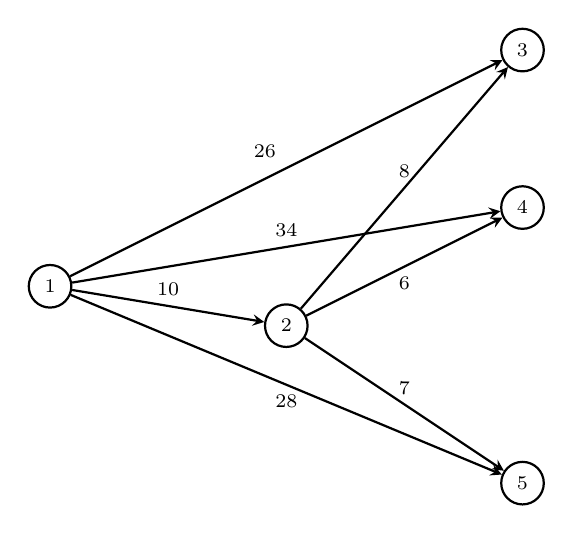
\begin{tikzpicture}
          [font=\scriptsize,
          node/.style={shape=circle,draw=black,fill=white!20, text=black,minimum width=0.5cm,thick},
          arc/.style={->,>=stealth,thick},
          edge/.style={thick}]

            \node (1) [node] at (0,0) {1};
            \node (2) [node] at (3,-0.5) {2};
            \node (3) [node] at (6,3) {3};
            \node (4) [node] at (6,1) {4};
            \node (5) [node] at (6,-2.5) {5};

          \draw [arc] (1) to node [pos=0.5,above] {10} (2);
            \draw [arc] (1) to node [auto] {26} (3);
            \draw [arc] (2) to node [pos=0.5,above] {8} (3);
            \draw [arc] (1) to node [above] {34} (4);
            \draw [arc] (2) to node [pos=0.5,below] {6} (4);
            \draw [arc] (2) to node [pos=0.5,above] {7} (5);
            \draw [arc] (1) to node [pos=0.5,below] {28} (5);

        \end{tikzpicture}
\end{center}

\noindent The net supplies $b_i=s_i - d_i$, where $s_i$ is the supply and $d_i$ is the demand at node $i$, for the nodes are given in the following table:

\begin{center}
\begin{tabular}{lccccc}
node & 1 & 2 & 3 & 4 & 5\\
\hline
$b_i$ & 3 & 0 & -1 & -1 & -1\\
\hline
\end{tabular}
\end{center}

\noindent The carrying capacity of the arcs $u_{ij}$ is given in the following table:

\begin{center}
\begin{tabular}{lccccccc}
arc & (1,2) & (1,3) & (1,4) & (1,5) & (2,3) & (2,4) & (2,5) \\
\hline
$u_{ij}$ & 3 & 1 & 1 & 1 & 1 & 1 & 1\\
\hline
\end{tabular}
\end{center}
For the questions that follow, use the decision variables $x_{ij}$ to indicate the amount of flow on arc $(i,j)$ and
binary variables $y_{ij}$, where $y_{ij} = 1$  if arc $(i,j)$ is to be used, and 0 otherwise, for all arcs $(i,j)$.

\begin{parts}
\part Write an objective function that seeks to minimize the cost of providing connectivity to all three customers.
\begin{solution}
\[
\min 10 y_{12} + 26 y_{13} + 34 y_{14} + 28 y_{15} + 8 y_{23} + 6 y_{24} + 7 y_{25}
\]
or
\[
\min \sum_{(i,j) \in A} f_{ij} y_{ij}
\]
where $A$ is the set of arcs given in the table above
\end{solution}

\part  Write the balance of flow constraint for node 2.

\begin{solution}
\[
x_{23} + x_{24} + x_{25} - x_{12} = 0
\]
or
\[
\sum_{j|(2,j) \in A} x_{2j} - \sum_{j|(j,2) \in A} x_{j2} = 0
\]
where $A$ is the set of arcs given in the table above
\end{solution}
\part  Write a constraint that ensures the flow from the backbone node (node 1) to the optical repeater (node 2) meets the following criteria:  is only nonzero if we pay to use arc $(1,2)$ in the objective function, and does not exceed the carrying capacity of arc $(1,2)$.

\begin{solution}
\[
x_{12} \le 3 y_{12}
\]
\end{solution}
\part  A new cost is introduced into the problem:  a fixed charge of 5 for using node 2, the optical repeater.  Modify the model to incorporate this new cost, including any changes to the objective function and/or constraints.  Define any new notation that you use.
\begin{solution}
Let $z_2$ denotes a binary variable that has value 1 if node 2 is used and 0 otherwise.\\
The objective function changes to the following for
\[
\min 10 y_{12} + 26 y_{13} + 34 y_{14} + 28 y_{15} + 8 y_{23} + 6 y_{24} + 7 y_{25}+5z_2
\]
We also need to add either a weak constraint or strong constraints for node 2. \\
Weak constraint: 
\[
x_{23}+x_{24}+x_{25} \leq 3z_2
\]

Strong constraints:
\[
x_{23} \leq 3z_2
\]
\[
x_{24} \leq 3z_2
\]
\[
x_{25} \leq 3z_2
\]
Note: Alternatively, we could have used incoming arcs for  node 2 to formulate  weak and strong constraints. Balance of flow constraint at node 2 will ensure that using incoming arcs  will produce the same results as using outgoing arcs. Since we have only one incoming arc, weak and strong constraints are the same.

Weak and strong constraint:
\[
x_{12} \leq 3z_2
\] 
Hence, it is more beneficial to use the second option with incoming arc $(1,2)$. 
\end{solution}



\end{parts}

\question You are trying to decide where you want to attend graduate school.  You plan to leave from and return to USNA after visiting each school one time.  You can visit the schools in any order, but you would like to determine a route of shortest total length.  A table of the corresponding distances, $d_{ij}$, from city $i$ to city $j$ is given in the  table below, with city 1 representing Annapolis.

\begin{center}
\begin{tabular}{l||c|c|c|c|c|c|c}
  & 1 & 2 & 3 & 4 & 5 & 6 & 7  \\
\hline
\hline
1   & 0 & 8 & 9 & 11 & 17 & 12 & 3 \\
\hline
2  & 8 & 0 & 11 & 5 & 6 & 10 & 7 \\
\hline
3  & 9 & 11 & 0 & 2 & 7 & 8 & 13 \\
\hline
4  & 11 & 5 & 2 & 0 & 3  & 4 & 4 \\
\hline
5  & 17 & 6 & 7 & 3 & 0  & 9 & 1 \\
\hline
6  & 12 & 10 & 8 & 4 & 9 & 0  & 6 \\
\hline
7  & 3  & 7 & 13 & 4 & 1 & 6 & 0\\
\hline
\end{tabular}
\end{center}

%\begin{center}
%  \begin{tikzpicture}
%    [font=\scriptsize,
%    node/.style={shape=circle,draw=black,minimum width=0.5cm,thick},
%    arc/.style={->,>=stealth,thick},
%    arclabel/.style={midway,sloped,above},
%    edge/.style={thick}]
%
%
%    \node (1) [node] at (-4,3) {1};
%    \node (2) [node] at (0,3) {2};
%    \node (3) [node] at (-4,0) {3};
%    \node (4) [node] at (0,0) {4};
%    \node (5) [node] at (-2,5) {5};
%    \node (6) [node] at (-2,-2) {6};
%
%    \draw [edge] (1) to node [above] {$20$} (2);
%    \draw [edge] (1) to node [left] {$42$} (3);
%    \draw [edge] (1) to node [auto, near start] {$35$} (4);
%    \draw [edge] (1) to node [above] {$7$} (5);
%    \draw [edge] (2) to node [above] {$7$} (5);
%    \draw [edge] (2) to node [auto, near start] {$30$} (3);
%    \draw [edge] (2) to node [right] {$34$} (4);
%    \draw [edge] (3) to node [above] {$12$} (4);
%    \draw [edge] (3) to node [left] {$7$} (6);
%    \draw [edge] (4) to node [right] {$7$} (6);
%
%  \end{tikzpicture}
%\end{center}
\begin{parts}
\part Write an abstract model whose solution provides a minimal cost way to begin at city 1, visit each of the other cities exactly one time each, and return to city 1.  Be sure to define any notation used in the model.
\begin{solution}
This is a traveling salesperson problem. We define the following:

\textbf{\underline{Sets}}\\
Let $V$ be the set of nodes \\
Let $E$ be the set of edges

\textbf{\underline{Decision Variables}}\\
Let $x_{i,j} = 1$ if edge $(i,j)$ is included in the tour and 0 otherwise for all $(i,j) \in E$

\textbf{\underline{Parameters}}\\
Let $d_{i,j}$ be the distance between cities $i$ and $j$ for all $(i,j) \in E$

\textbf{\underline{Objective function}}\\
\[
\text{min distance: } \sum_{(i,j) \in E} d_{i,j} x_{i,j}
\]

\textbf{\underline{Constraints}}\\
\begin{optprog*}
& \sum_{ (r,j) \in E} x_{r,j} + \sum_{ (i,r) \in E} x_{i,r} & = & 2 & \text{for all $r  \in V$} \\
& \sum_{ (i,j) \in S} x_{i,j} & \leq & \vert S \vert -1 & \text{for all $S \subset V$, $\vert S \vert  \geq 3$} \\
& x_{i,j} & \in & \{0,1\} & \text{for all $(i,j) \in E$}
\end{optprog*}



\end{solution}
\part Provide a concrete example of each type of constraint that appears in the abstract model.  Explain the purpose and logic of each of the example constraints.
\begin{solution}
For the first constraint consider node 1. We have:
\[
x_{1,2} + x_{1,3} + x_{1,4} + x_{1,5} + x_{1,6} + x_{1,7} = 2
\]

The logic of this constraint is that every node is touched exactly twice by an edge. Essentially this means that each node is visited and left in the tour. Additionally, no node is visited more than once.

The second constraint, consider a set of size 3 on nodes 1, 2, and 3. We would have:
\[
x_{1,2} + x_{1,3} + x_{2,3} \leq 2
\]

This constraint ensures that no cycle is formed on the three nodes 1, 2, and 3 because it is impossible to form a cycle on 3 nodes with only two edges.


\end{solution}
\part Write the concrete constraint(s) from the abstract model from part (a) that would prevent a solution that includes a tour among cities 1, 4, and 5, and a separate tour among the rest of the cities.
\begin{solution}
\[
x_{1,4} + x_{1,5} + x_{4,5} \leq 2
\]

This ensures a separate cycle is not formed just on nodes 1, 4, and 5.

\end{solution}
\end{parts}

\newpage
\question The city of Examopolis has hired you to help them decide where to place some new emergency response facilities.  The figure below will be used to help make the decision, where each of the $n=9$ nodes $I = \{1,2,...,9\}$ correspond to the boroughs who need service and the nodes $J=\{3, 5, 6, 9\}$ in dashed boxes are the possible emergency response facility locations.  The weight on each edge $(i,j)$ corresponds to direct distance between $i$ and $j$.  Let the distance $d_{ij}$ be the length of the shortest path in this graph between nodes $i$ and $j$.
\begin{center}
  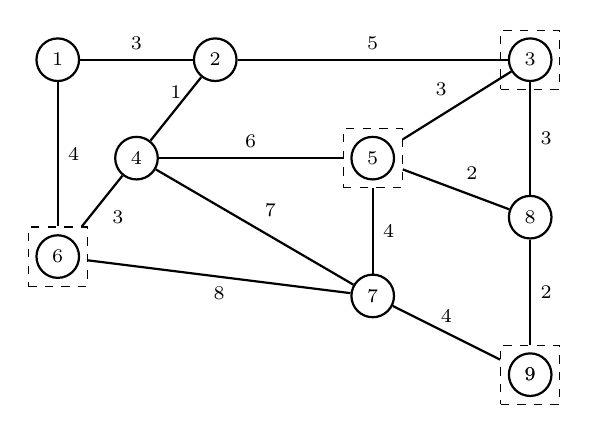
\begin{tikzpicture}
    [font=\scriptsize,
    %    node/.style={shape=circle,draw=blue!60,fill=blue!20,minimum width=0.5cm,thick},
    node/.style={shape=circle,draw=black,minimum width=0.5cm,thick},
    node1/.style={shape=rectangle,draw=black,minimum width=0.75cm,minimum height=0.75cm,dashed},
    arc/.style={->,>=stealth,thick},
    edge/.style={thick}]

    \node (1) [node] at (-2,2) {1};
    \node (2) [node] at (0,2) {2};
    \node (3) [node1] at (4,2){};
    \node (3) [node] at (4,2) {3};
    \node (4) [node] at (-1,0.75) {4};
    \node (5) [node] at (2,0.75) {5};
    \node (5) [node1] at (2,0.75){};
    \node (6) [node] at (-2,-0.5) {6};
    \node (6) [node1] at (-2,-0.5){};
    \node (7) [node] at (2,-1) {7};
    \node (8) [node] at (4,0){8};
    \node (9) [node] at (4,-2) {9};
    \node (9) [node1] at (4,-2) {9};

    \draw [edge] (1) to node [auto] {3} (2);
    \draw [edge] (1) to node [auto] {4} (6);
    \draw [edge] (2) to node [auto] {5} (3);
    \draw [edge] (2) to node [above] {1} (4);
    \draw [edge] (4) to node [auto] {6} (5);
    \draw [edge] (4) to node [auto] {3} (6);
    \draw [edge] (4) to node [auto] {7} (7);
    \draw [edge] (5) to node [auto] {3} (3);
    \draw [edge] (5) to node [auto] {4} (7);
    \draw [edge] (5) to node [auto] {2} (8);
    \draw [edge] (3) to node [auto] {3} (8);
    \draw [edge] (6) to node [below] {8} (7);
    \draw [edge] (7) to node [above] {4} (9);
    \draw [edge] (8) to node [auto] {2} (9);

  \end{tikzpicture}
\end{center}

\noindent The city council has asked that you use the following notation when formulating your responses to their questions.

\begin{tabbing}
\noindent{\bf Indices and Sets}\\[0.2cm]
\hspace*{.25cm} \= $i\in I$ \hspace{0.3cm} \= boroughs, $I=\{1,2,...,9\}$ \\
\> $j\in J$ \> possible emergency response facility locations, $J=\{3,5,6,9\}$\\[0.2cm]
\noindent{\bf Data}\\[0.2cm]
\> $h_i$ \> population at node $i$ in thousands\\
\> $D$ \> maximum allowable distance between a borough and its servicing facility \\
\> $N_i$ \> neighborhood of $i$, where $N_i = \{ j  \in J : d_{ij} \leq D \}$  is the set of all facilities $j$\\
\>            \> that can serve node $i$ \\
\> $d_{ij}$ \> the length of the shortest path between node $i$ and node $j$ \\[0.2cm]
\noindent{\bf Decision Variables}\\
\> $x_j$ \> 1 if node $j$ is the location of an emergency response facility, 0 otherwise\\
\> $y_{ij}$ \> 1 if borough $i$ has its demand satisfied by emergency response facility $j$, 0 otherwise\\[0.2cm]
\end{tabbing}

\begin{parts}
\part Write an objective function that minimizes the number of emergency response facilities needed.

\begin{solution}
\[
\min \sum_{j \in J} x_{j}
\]
\end{solution}


\part If $D = 7$, write out all the elements of $N_4$.

\vspace{0.2cm}

\begin{solution} $N_4 = \{ 3, 5, 6 \}$
\end{solution}

\part Write a set of constraints which ensures each borough must be associated with an emergency response facility in its neighborhood, $N_i$.

\begin{solution}
\[
\sum_{j \in N_i} x_{j} \geq 1, ~~ i \in I
\]
\end{solution}

\vfill

\noindent
The city council now wants a model that attempts to minimize the maximum distance between a borough and its closest emergency response facility.
\vspace{0.2cm}

\part Let $W$ be the maximum distance between a borough $i$ and its assigned facility $j$.  Write an objective function and corresponding set of constraints that minimizes this maximum distance.

\begin{solution}
\begin{equation}
  \begin{array}{lll}
    \min & W & \\
    \mbox{s.t.} & \sum_{j \in J} d_{ij} y_{ij} \leq W, & i \in I  \nonumber
  \end{array}
\end{equation}

or

\begin{equation}
  \begin{array}{lll}
    \min & W & \\
    \mbox{s.t.} & d_{ij} y_{ij} \leq W, & i \in I, ~ j \in J  \nonumber
  \end{array}
\end{equation}
\end{solution}





\part Write a constraint which ensures exactly 2 emergency response facilities are opened.

\begin{solution}
\[
\sum_{j \in J} x_j = 2
\]
\end{solution}

\part Write a set of constraints which ensure that borough $i$'s demand is met by emergency response facility $j$ only if facility $j$ is open.

\begin{solution}
\[
y_{ij} \leq x_j,~~i \in I, ~ j \in J
\]
\end{solution}
 \part Write one or more constraints to ensure that if a facility is opened at either 3 or 9, then a facility must not be opened at 5.  The constraint(s) should not impose any restriction on the facility at 5 if neither 3 nor 9 are opened.
 \begin{solution}
 $x_5 \leq 1 - x_3$, $x_5 \leq 1 - x_9$
 \end{solution}

\end{parts}


\end{questions}

\end{document}


%\question  The goal of the famous graph coloring problem is to find the minimum number of colors required to color the vertices of a graph so that no two adjacent vertices have the same color.  For this single-color variation on graph coloring, we  want to color as many vertices ``red'' as possible, without coloring adjacent vertices.  Consider the graph below.  Let $x_i = 1$ if vertex $i$ is colored red, and 0 otherwise.

%\begin{center}
%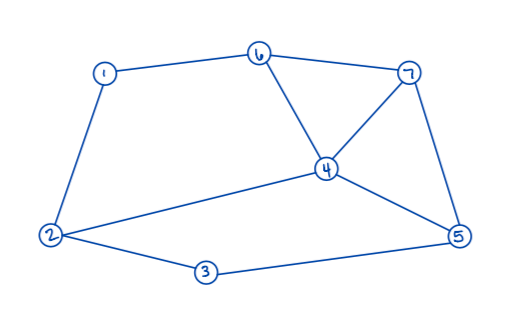
\includegraphics[width=0.5\textwidth]{graph1}
%\end{center}

%\begin{parts}
%\part Formulate a concrete objective function, as well as a set of concrete constraints that enforce the logic that at most one of any pair of adjacent vertices can be selected.  (For example, at most one of 4 and 6 can be selected.)
%\part Write the model in abstract form.  Define any sets that are required.  (You shouldn't need any parameters.)
%\end{parts}
